\chapter{Trabajo Realizado}
\label{chap:trabajo}
El trabajo realizado a lo largo del semestre se puede dividir en dos secciones principales: la realización de simulaciones y la escritura de códigos de análisis y comparación para dichas simulaciones. Para el primer caso implica la lectura de cómo correr las simulaciones en clusters de múltiples procesadores, definir los parámetros de instalación y de simulación en sí y observar los comportamientos, tiempos de duración y modos de exportación de datos de cada simulación. Para la segunda sección se incluyen los códigos realizados y utilizados que permiten desde la lectura de los datos brutos de simulación hasta la extracción de propiedades y generación de gráficas de análisis. A continuación se explicarán las diferentes secciones y detalles del trabajo realizado, así como los resultados de dicho trabajo.

\section{Características de Simulación}
Los datos manejados a lo largo del proyecto son $100\%$ provenientes de simulaciones computacionales, de manera que la correcta planeación, manejo y ejecición de dichas simulaciones es vital para los resultados. A continuación se describen las características de la instalación y ejecución de las simulaciones realizadas.

\subsection{Parámetros de instalación y compilación}
Para correr una simulación en Gadget-2 se requiere principalmente de 3 librerías previamente instaladas y de un set de condiciones iniciales sobre las cuales trabajar. Las tres librerías que se deben instalar son FFTW, GSL y MPI, todas ellas de libre distribución e instalación. FFTW es una librería, o conjunto de librerías, con códigos para la realización de transformadas de Fourier en espacio discreto, como la transformada rápida de Fourier (FFT), cuyo uso se explicó en la Sección \ref{sub:gadget}. GSL (\textit{GNU Scientific Library}) como su nombre lo dice es una librería con un gran conjunto de funciones de uso científico. Finalmente, MPI (\textit{Message Passing Interface}) es la librería de instrucciones, rutinas y métodos para la paralelización de procesos en múltiples procesadores. 

Una vez instaladas las librerías se procede a compilar los ejecutables, para lo cual es necesario configurar el MakeFile. En éste se comentan las características y utilidades que no se requieren usar de Gadget-2, así como se activan las que sí. Para el caso del proyecto, los puntos más importantes del MakeFile son activar las condiciones de frontera periódicas, activar el mallado PM (para el algoritmo TreePM explicado en la Sección \ref{sub:gadget}), el uso de Peano-Hilbert para la paralelización y desactivar el uso de librería HDF5, la cual no fue instalada. Finalmente, se indica las ubicaciones de las librerías previamente instaladas, lo cual cambia dependiendo de la arquitectura del sistema y se procede a compilar para generar el ejecutable de la simulación. Este proceso es idéntico para Gadget-2 y para N-GenIC, que es el código utilizado para el tercer requerimiento: las condiciones iniciales. N-GenIC es un código de generación de condiciones iniciales que a partir de un archivo \textit{glass} de partículas homogéneamente distribuidas en un mallado genera un archivo del tipo snapshot de Gadget-2 con una distribución de masas y velocidades homogénea. El archivo \textit{glass} utilizado tenía un total de $16^3$ partículas de manera que de acuerdo a los requerimientos de la simulación (número total de partículas) se puede apilar una cierta cantidad de archivos en cada eje, o crear uno de mayor tamaño.

Como se explicará más a fondo en la Sección \ref{sub:simulaciones}, las simulaciones fueron realizadas no sólo en computadores personales sino que también se hizo uso del clúster de física de la Universidad de los Andes y además se corrieron las simulaciones definiticas en el clúster KIAS en Corea, para lo cual fue necesario la conexión y ejecución de comandos remotos mediante la terminal de Ubuntu. Mediante el comando \textit{ssh}, con un usuario y una clave, se establece una conexión remota con el clúster o máquina en cuestión que permite correr cualquier comando o script. En el caso de la ejecución de las simulaciones es importante tener en cuenta la arquitectura y manejo que tenga cada clúster, puesto que en un clúster de bajo uso como lo era el Fiscluster se podía ejecutar directamente el script de la simulación en los nodos que estuviesen desocupados, siempre y cuando los resultados de simulación quedasen dentro de las limitaciones de espacio de disco duro y computación. En cambio, para un cluster de mayor nivel de organización e infraestructura como lo es KIAS, hay que cumplir con una serie de recursos máximos permitidos y además el script no puede ser ejecutado directamente, sino que debe contener la información de la cantidad de nodos y procesadores requeridos y correr el comando \textit{qsub} con el scrip. Este comando añade el script a un sistema de colas, para el cual el administrador de colas, en base a los requerimientos descritos para el script, asigna los procesadores en los que correrá el proceso. Esta organización permite una mejor distribución de los recursos, evitando la sobrecarga de algún nodo. El estado del proceso puede ser seguido mediante el comando \textit{qstat} el cual muestra los procesos corriendo por el usuario actual y con el comando \textit{qhost} que muestra el estado actual de uso de los recursos del clúster, como la carga de los nodos y la memoria usada. 

Dado que en el clúster no se hacía uso de las colas de trabajo y los scripts se corrían directamente desde la consola, en el caso de haber una desconexión del computador y romper el acceso remoto, las simulaciones se detenían. Para corregir este problema se hizo uso del comando \textit{nohup} el cual permitía que el código se siguiese ejecutando sin necesidad de la conexión permanente por consola, así todos los outputs que normalmente aparecerían en la consola se guardaban en un archivo de texto.

\subsection{Parámetros de la simulación}
Una vez se tiene listo el ejecutable, se prepara el script para la ejecución de la simulación, mediante el comando \textit{mpirun} o \textit{mpiexec} los cuales deben recibir como entrada el número de procesadores en los que se va a correr la simulación, un archivo con la lista específica de los nodos a usar, el ejecutable y cualquier entrada que requiera dicho ejecutable. Tanto para el caso de N-GenIC como para Gadget-2 se requiere un archivo de parámetros en el cual se especifican las condiciones de simulación, la ubicación de datos de entrada y datos de salida y los parámetros cosmológicos, entre otros. 

Los datos más importantes para tener en cuenta con el archivo de parámetros de N-GenIC son: los parámetros cosmológicos $\Omega$, $\Omega_\Lambda$, $\Omega_b$, $H$, $\sigma_8$; el \textit{redshift} inicial de la simulación, $z$; el tamaño de la caja, en kiloparsecs; el \textit{TileFac}, que corresponde al número de veces que se replica el archivo \textit{glass} en cada dirección (\textit{i.e.} número de partículas); y los parámetros de escritura y lectura, como carpetas y bases para nombres de exportación. El parámetro cosmológico $\sigma_8$ es el cual determina cómo son las fluctuaciones de densidad en el universo, debido a que da cuenta de qué tan dispersas o desviadas son dichas fluctuaciones en esferas de $8Mpc$, de manera que como se puede observar en la Figura \ref{fig:sigma}, en una simulación con un $\sigma_8$ mayor, habrá un mayor contraste (serán más pronunciadas las fluctuaciones) de densidades. 

\begin{figure}
	\centering
	\begin{subfigure}[b]{0.49\textwidth}
		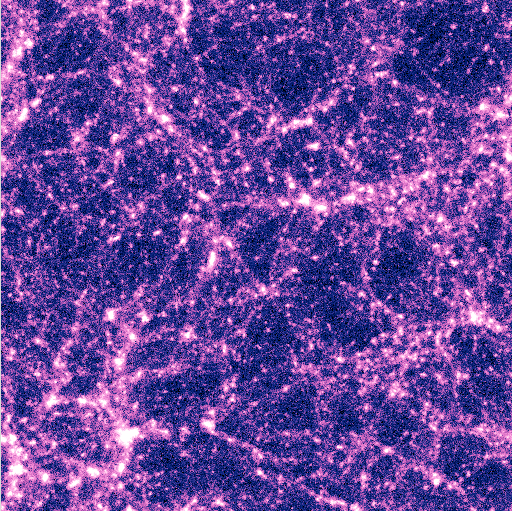
\includegraphics[width=\textwidth]{Trabajo/res1}
		\caption{$\sigma_8=0.9$}
		\label{fig:sig9}
	\end{subfigure}
	\begin{subfigure}[b]{0.49\textwidth}
		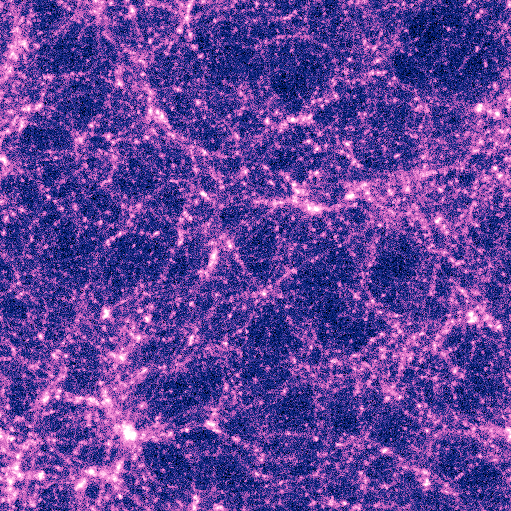
\includegraphics[width=\textwidth]{Trabajo/res2}
		\caption{$\sigma_8=0.7$}
		\label{fig:sig7}
	\end{subfigure}
	\caption[Dos simulaciones de $128^3$ partículas con iguales condiciones a excepción de $\sigma_8$.]{Dos simulaciones de $128^3$ partículas con iguales condiciones a excepción de $\sigma_8$. También se aprecian las condiciones periódicas de la simulación.}
	\label{fig:sigma}
\end{figure}

En cuanto al archivo de parámetros de Gadget-2 es un poco más extenso, pero la esencia se conserva, comenzando porque se deben volver a incluir los parámetros cosmológicos y el tamaño de la caja, para lo cual no sobra recordar que dichos valores deben coincidir con los utilizados en el archivo de parámetros de las condiciones iniciales. Nuevamente se deben especificar detalles acerca de la importación de condiciones iniciales (resultados de N-GenIC) y exportación de estados parciales, resultados y archivos de reinicio para cada procesador. Gadget exporta los resultados parciales y totales en archivos de estados donde se tienen todos los datos de la simulación actual en un punto dado; este archivo se explica más a fondo en la Sección \ref{sub:snap}. En el archivo de parámetros se deben incluir nuevamente los tiempos de inicio de la simulación, pero esta vez en términos del parámetro de dilatación $a=\frac{1}{1+z}$ y además el tiempo del primer snapshot y el intervalo de tiempo de cada cuando debe exportarse un snapshot (ya sea por un factor aditivo o multiplicativo). Entre otros parámetros para modificar se encuentran el tiempo máximo de simulación, los errores y tolerancias de los métodos de Tree BH y SPH. Finalmente se tienen las distancias de \textit{softening}, para las que se aconseja usar un décimo del equivalente a la distancia media libre.

\subsection{Simulaciones realizadas}
\label{sub:simulaciones}
A lo largo del desarrollo del proyecto se corrieron múltiples simulaciones con diferentes características y propósitos, desde las simulaciones de prueba, las cuales permitían observar si el código corría correctamente, hasta las simulaciones definitivas en donde lo más importante eran las variables de entrada. Inicialmente, para la familiarización con el entorno de ejecución y con los modos de ejecución, se corrieron simulaciones de prueba en un computador portátil, lo cual daba para un máximo de dos procesadores. Una vez comprobado que el método de compilación y ejecución de Gadget-2 y N-GenIC era el correcto se procedió a instalar nuevamente las librerías en el clúster del Departamento de Física de la Universidad de los Andes, \textit{fiscluster}. Una vez listas, se corrieron las primeras simulaciones para $128^3$ partículas, cuyos resultados corresponden a la Figura \ref{fig:sigma}. Estas primeras simulaciones fueron realizadas en una caja periódica de tamaño de $150Mpc$ y tomaron aproximadamente 3 horas de cómputo en 32 procesadores. Para estas primeras simulaciones, cada snapshot exportado por Gadget-2 pesaba alrededor de $57Mb$. En la Figura \ref{fig:escala} se puede apreciar una escala del tamaño de la caja en las simulaciones definitivas respecto a las simulaciones de prueba.

\begin{figure}
	\centering
	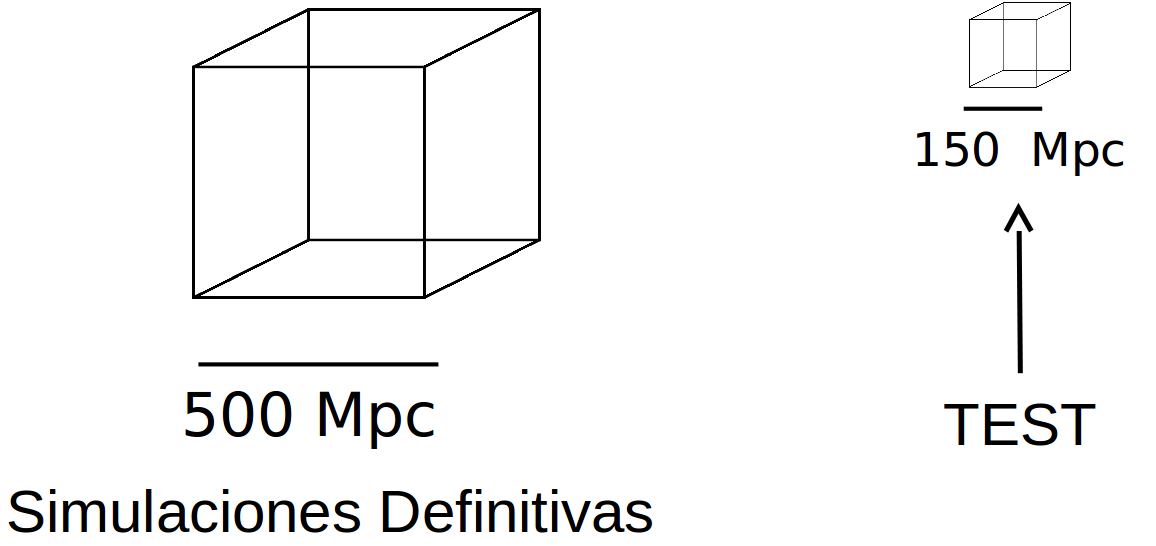
\includegraphics[width=0.6\textwidth]{Trabajo/escala}
	\caption{Comparación de tamaños entre simulaciones de prueba y simulaciones definitivas}
	\label{fig:escala}
\end{figure}

El siguiente paso a seguir fue realizar simulaciones de $256^3$ partículas en una caja periódica de $500Mpc$ de lado, pero esta vez variando el parámetro de $\Omega$ de $0.3$ a $0.35$. El tiempo de simulación tomado para estas simulaciones fue de aproximadamente 24 horas corriendo en 40 procesadores. Debido a la gran cantidad de partículas en la lista, cada snapshot generado para este segundo grupo de simulaciones pesó $449Mb$. Para el grupo definitivo de simulaciones realizadas se tomó nuevamente la caja de $500Mpc$, pero nuevamente se aumentó el número de partículas en un factor de 8, dando así un total de $512^3$ partículas; $64$ veces más que en las simulaciones de prueba. El tamaño final de cada snapshot generado para esta cantidad de partículas fue de $3.6Gb$. Para este último grupo de simulaciones hubo una limitación de memoria física para correr la simulación, incluso corriendo en el máximo de 56 procesadores en fiscluster, no fue posible completar las simulaciones. Fue por esta razón que se decidió migrar la simulación al clúster KIAS en Corea, con una capacidad de 256 procesadores. 

El migrar de clúster implicó reinstalar las librerías necesarias para la simulación y también correr nuevamente simulaciones pequeñas para entender el modo de funcionamiento de los trabajos. Este clúster funciona con un sistema de colas de trabajos, de manera que los scripts ser presentados a un administrador de colas quien se encarga de ejecutarlos. Una vez en proceso, se crean dos archivos con radical igual al script, en donde se puede realizar el seguimiento del output de la ejecución (para el primero) y los posibles errores (en el segundo). El cambio de clúster supuso una notoria mejoría en los tiempos de ejecución, puesto que para la creación de las condiciones iniciales se debían realizar en un único procesador, pues Gadget-2 tiende a tener errores al leer un archivo de condiciones iniciales dividido. Así, en fiscluster la creación de estos archivos tomaba alrededor de 20 minutos o más, mientras que en KIAS dicho proceso tomó 5 minutos. Las simulaciones definitivas tomaron aproximadamente 4 días en total, y los parámetros usados para dichas simulaciones se muestran en la Tabla \ref{tab:param} y son datos tomados del proyecto Plank.

\begin{table}[H]
	\centering
	\begin{tabular}{cc}
		\hline \hline
		\textbf{Parámetro} & \textbf{Valor} 		\\
		\hline
		$\Omega_0$ 			& $0.3175\pm0.05$ 	\\
		$\Omega_\Lambda$ 	& $0.6825 \mp 0.05$	\\
		$\Omega_b$ 			& $0.048$			\\
		$H$					& $0.6711$			\\
		$\sigma_8$			& $0.834$			\\
		\hline
	\end{tabular}
	\caption{Parámetros de simulaciones definitivas}
	\label{tab:param}
\end{table}

\section{Códigos de Análisis}
Una vez realizadas las simulaciones, es necesario crear códigos y programas que permitan la extracción de la información necesaria para los propósitos del proyecto. En la siguiente sección se describen brevemente los códigos creados para dicho propósito. Los algoritmos de análisis siguieron dos ramificaciones principales: el análisis por densidades y el análisis por halos. Para el segundo se tiene un proceso de búsqueda y clasificación de halos para un posterior análisis transversal de las simulaciones. Los lenguajes de programación usados fueron principalmente C para la extracción de información y análisis de la misma y Python (más exactamente la utilidad de IPython notebook) para la generación de gráficas.
\subsection{Estructura del \textit{Snapshot}}
\label{sub:snap}
Los snapshots de Gadget-2 están escritos en binario, lo cual permite una velocidad de escritura mayor y a su vez un menor consumo de memoria física. Para la lectura de los snapshots se utilizó el código \textit{read\underline{\hspace{.1in}}snapshot.c} el cuál se encuentra en la carpeta de Analysis de la instalación de Gadget-2. Este código permite la lectura el snapshot y la extracción de las posiciones y velocidades de cada partícula en cada eje, de manera que los posteriores códigos tengan acceso a dicha información para su análisis. 

El snapshot inicia con un encabezado en el cual indica la cantidad de partículas que hay en cada tipo de los 6 cuerpos manejados por Gadget-2, estos son: gas, halo, disco, \textit{bulge}, estrella y frontera. Los siguientes 6 datos en el encabezado indican la masa asignada a cada tipo de cuerpo, la cual varía debido a que se busca una densidad homogénea y se varía el número de partículas y el tamaño de la caja. Los datos de masa en el snapshot están dados en unidades de $10^{10}M_{\odot}$. A continuación se listan ciertos parámetros del estado de simulación, como lo son el tiempo, el redshift, el tamaño de la caja y los parámetros cosmológicos. Una vez terminado el encabezado, comienza el listado de partículas primero indicando la posición en tres coordenadas de cada una, en unidades de kiloparsec. Una vez se termina el listado de posiciones, inicia el listado de velocidades en tres dimensiones, en $km/s$. Finalmente, se realiza un nuevo listado con el número de identificación ID de cada partícula. El código también permite realizar una conversión de unidades de energía y una reorganización de partículas de acuerdo a si número de identificación.

\subsection{Extracción de Halos}
Para la extracción de los halos se hizo uso del código HackFOF el cual utiliza el algoritmo de \textit{Friend of Friends} (FoF) para identificar los halos de materia oscura. Para este algoritmo se define un linking lenght, el cual se definió aproximadamente como $0.2$ veces la distancia media esperada entre partículas, y se procede a recorrer las partículas, buscando para cada una cuales caen dentro de una esfera de dicho radio. Una vez encontrada la lista que cumplen con dicha condición, se repite el proceso con las partículas en dicha lista, y así hasta que no se agregue ninguna partícula nueva a la lista, y la lista resultante es un halo de materia oscura. 

Para la utilización de este código, se debe exportar previamente un archivo de texto con la información de las partículas (posiciones en tres dimensiones separadas por un espacio), precedido por un encabezado similar al del snapshot, en el que se indican el número total de partículas, el número total de partículas tipo halo, en número de partículas tipo gas, el número de partículas tipo estrella, el tiempo y un factor llamado \textit{nactive}, que para efectos del proceso se le asigna cero. Cuando este archivo es exportado se puede proceder a ejecutar el código FoF haciendo uso de las banderas para el uso de la opción de condiciones periódicas. 

Una vez terminado de correr el FoF, éste exporta un nuevo archivo que contiene la información de la cantidad total de partículas, seguido por una lista con el índice del halo correspondiente a la partícula en dicha posición; los índices correspondientes a las partículas están en el mismo orden de las partículas ingresadas a HackFOF. El índice cero significa que la partícula no está asignada a ningún halo, mientras que cualquier otro índice indica el número del halo. Este archivo es cargado nuevamente para realizar un análisis del número de halos existentes en la simulación y calcular los centros de masa y velocidades de centro de masa respectivos para cada uno. Para las simulaciones de $128^3$ partículas se encontraron alrededor de $6000$ halos, para la simulación de $256^3$ aproximadamente $70000$ halos y \textcolor{red}{para las simulaciones definitivas de $512^3$ partículas se encontraron aproximadamente $ $ halos}.

\subsubsection{Identificación de correspondencias}

Dado que la idea del proyecto es observar cambios en los universos simulados, fue necesario encontrar halos correspondientes entre las simulaciones. Esto es posible ya que en el archivo de parámetros de la generación de condiciones iniciales, uno de los parámetros corresponde a una semilla de generación de números aleatorios y al dejar esta semilla invariante, los universos tendrán estructuras y comportamientos similares. Para la búsqueda de estos halos correspondientes, se realiza un recorrido a través de los halos de la simulación de referencia (aquella con los valores de Plank) y para cada halo se busca dónde están las partículas correspondientes en las demás simulaciones, finalmente se selecciona aquel con mayor número de coincidencias, claro está, siempre y cuando sea un valor razonable. 


\subsection{Campo de densidades (CIC)}
\label{sub:CIC}
El cálculo del campo de densidades de la simulación y la sobredensidad en cada punto es la segunda vertiente del código, pero que para los efectos finales del proyecto complementa los datos de la primera vertiente. 


\section{Análisis y Resultados}
